\documentclass{article}

% required includes
\usepackage{graphicx}
\usepackage{url}

\usepackage{tikz}
\usetikzlibrary{shapes,arrows}
% styles for flowcharts
\tikzstyle{machine} = [star, star points=7, star point ratio=0.8, draw, text width=5em, text badly centered, node distance=3cm, inner sep=0pt]
\tikzstyle{data} = [trapezium, trapezium left angle=70, trapezium right angle=-70, draw,text centered]
\tikzstyle{process} = [rectangle, draw, text width=5em, text centered, rounded corners, minimum height=4em] 

\addtolength{\textwidth}{10pt}

\title{CAT-DWAM, A Question Answering System}
\author{
Alec Story,
Ansu Abraham,
Craig Frey,\\
Dustin Tiedemann,
Michael Zhu,
Thomas Levine,
Whitney Foster\\
}

\begin{document}
\maketitle

\section{Overview}

% What are you doing. Why are you doing it.
% ``this is effectively a statement of your hypothesis, so you should
% include justification of why you think that the particular approach
% will be effective

\section{The QA System}
% we need:
% a detailed walkthrough of what our system did to handle one question
% (in general) in the corpus. include the system output (enough to
% convince them that it is actually doing what we say)

% this is pretty much the final system proposal from part
% one. delete/rewrite if necessary (we need a description of the
% baseline in our final report)
We implemented our question answering system in Python, and use external
tools such as the natural language toolkit.

Our design mimics the design of Watson, with the intention of trying out a
variety of techniques to select answers from documents, and to use a machine
learning system to choose the appropriate one.  See figure \ref{diagram} for
a graphical overview.

We first shred the documents for each question into all of the component verb
and noun phrases.  We pass these candidates into a battery of evaluators that
assign a confidence value to each of them, and pass these confidences into a
machine learning algorithm that combines them to produce a ranked output.

From this ranked output we choose our final answers.

\begin{figure}
 \label{diagram}
 \begin{center}
  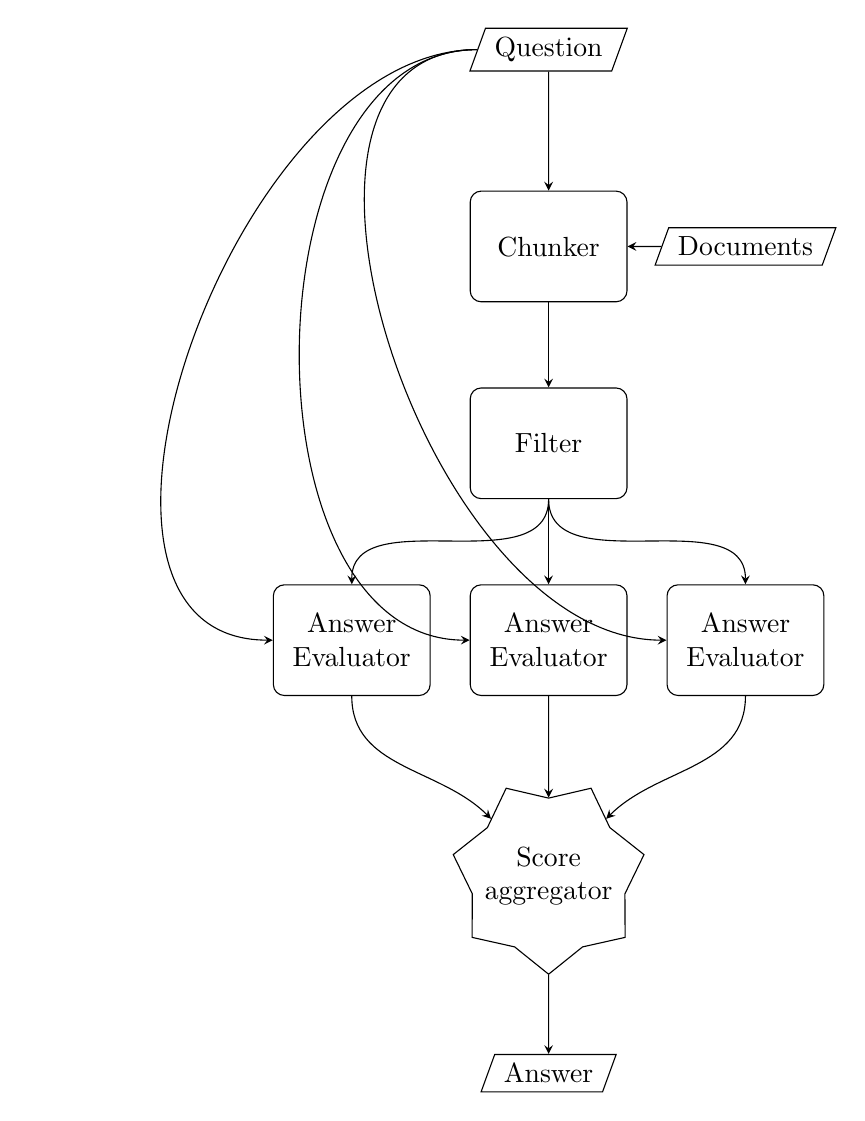
\begin{tikzpicture}[node distance=2.5cm, auto, >=stealth]
   % nodes
   \node[data] (Q)                                      {Question};
   \node[process] (ch) [below of=Q]                     {Chunker};
   \node[data] (docs) [right of=ch]                     {Documents};
   \node[process] (fil) [below of=ch]                     {Filter};
   \node[process] (a2) [below of=fil]                    {Answer Evaluator};
   \node[process] (a1) [left of=a2]                     {Answer Evaluator};
   \node[process] (a3) [right of=a2]                    {Answer Evaluator};
   \node[machine] (as) [below of=a2]                    {Score aggregator};
   \node[data] (A) [below of=as]                        {Answer};
   
   % edges
   	\draw[->] (Q) to (ch);
	\draw[->] (docs) to (ch);
	\draw[->] (ch) to (fil);
	\draw[->] (fil.south) to [out=270, in=90] (a1);
	\draw[->] (fil.south) to [out=270, in=90] (a2);
	\draw[->] (fil.south) to [out=270, in=90] (a3);
	\draw[->] (Q.west) to [out=180, in=180] (a1);
	\draw[->] (Q.west) to [out=180, in=180] (a2);
	\draw[->] (Q.west) to [out=180, in=180] (a3);
	\draw[->] (a1.south) to [out=270, in=135] (as);
	\draw[->] (a2.south) to [out=270, in=90] (as);
	\draw[->] (a3.south) to [out=270, in=45] (as);
	\draw[->] (as) to (A);
  \end{tikzpicture}
  \caption{Data Flow}
  \label{flowchart}
 \end{center}
\end{figure}

\subsection{Parsing the Corpus Documents}
% Talk about Whitney's Shredder module here
	To get candidate answers we took in the question number, parsed the
	documents associated with it by chunking it into syntactically correlated
	parts of words (noun phrases, verb phrase, etc), and outputted a list of
	tuple candidate answers.  These were in the format (string of candidate
	answer, document number, word index in the document, the phrase tag,
	question number). 

	To chunk the documents for the question, we prepared them by separating out
	the punctuation and the words with a space so that the taggers would work.
	We then POS tag all the words in the document and then get the IOB chunk
	tags for all the words. This data is then run through the conll.2000 chunker
	(http://www.clips.ua.ac.be/conll2000/chunking/) that labels what type of
	phrase the word belongs to (noun phrase, verb phrase, etc). The words in
	the same phrase are then combined together to form one long phrase as the
	candidate answer string.

\subsection{Answer Evaluators}

\subsubsection{Question-Document Comparison}

	We implemented a system to compare the question and answer against the
	proposed document in two ways:  one, with a na\"ive diffing algorithm that
	simply seeks out the longest indentical sequence, and one by implementing
	the Smith-Waterman local alignment
	algorithm.\footnote{\url{http://en.wikipedia.org/wiki/Smith-Waterman_algorithm}}
	We also implemented a system to attempt to re-write questions, discussed
	below, and applied these same techniques to the re-written question

	The na\"ive method does an adequate job when the document highly resembles
	the question, but does very poorly otherwise because it has no tolerance of
	faults.  The local alignment does much better for documents that resemble
	the question a great deal, but are not precise - it can smoothly deal with
	small differences, and still produce a good alignment.  This is a standard
	technique from bioinformatics, and is used extensively to align small
	sequences of DNA, RNA or protein against a larger corpus, such as a
	chromosome or a whole genome.  This is a fairly similar usage to aligning a
	question against a document which is much longer than the question.

	We chose Smith-Waterman over the similar Needleman-Wunsch, of which is a
	special case, because Needleman-Wunsch creates a \emph{global} alignment,
	which forces all of the characters in both strings to align.  This leads to
	the insertion of many gaps, and needlessly aligns words which are useless,
	for example, ``Who is Queen of England?'' should align well against
	``Elizabeth is Queen of England'' and it does, under Smith-Waterman, but the
	``who'' causes Needleman-Wunsch to choke.  Similarly, Needleman-Wunsch does
	not excuse one string for being shorter than the other, and chokes on all of
	the apparent gaps that it needs to insert, so it is not a good choice.

	We locate what we best believe to be the question via these two methods, and
	then evaluate how far away from that segment of the document the answer is.
	If it is fairly close, that is a good indicator that it is highly related to
	the question, but if it is far, it is likely to be unrelated.  We output
	that distance, and either the length of the na\"ive alignment or the score
	that Smith-Waterman produces (higher is better for both) because very short
	or very poor alignments are less likely to reflect an actual representation
	of the question.

\subsubsection{Punctuation}

	1 if the candidate answer is immmediately followed by a comma, period,
	quotation marks, semicolon, or exclamation mark, and 0 otherwise. This is a
	good heuristic by which to rank candidate answers since it retrieves a
	property from the context where the answer appears in the document.

\subsubsection{Apposition Filter}
% Alec

	Because we thought it would be difficult to analyze complete parse
	information for questions, we decided to tackle apposition by a simple
	heuristic:  does "question, answer," align better than "question answer"?
	If it does, then the answer is likely to be in apposition.  We also applied
	this to re-written questions.


\subsubsection{Number and Quantity Answer Type Filters}
% Tom
We used regular expressions to identify answer candidates that contained digits.
We classified these candidates as number-type answers or quantity-type answers.
Answer candidates containing exclusively digits were classified as number-type
answers, and answer candidates containing digits and other characters were classified
as quantity-type answers.

\subsubsection{Measurement Units or Matching Type Filters}
% Tom
For quantity-type answer candidates, we used simple regular expressions to extract
the proceeding and preceeding space-delimited phrases. This is quite close to a
lay definition of ``word''; for the answer candidate ``about 350 km/h'', the
phrases ``about'' and ``km/h'' would be extracted as units. We extracted the units
from the training corpus.

For test answers, we searched the context of the answer for colocated units
matching what we found in the training corpus. We returned a score of 1 if there
was a unit and a score of 0 if there wasn't.

\subsubsection{Sequence Length}
% Mike
This evaluation measures the difference between sequence length of the question
and the answer. It finds the length of the maximum sequence between the
question and answer and also finds the length of the maximum sequence between
the rewritten question and answer. A sequence is a list of (not necessarily 
consecutive) words that are shared by two sentences.

\subsubsection{Word Vector Comparison}

This evaluation measures the angle difference between the word vector of the
question and the answer, after removing stop words, and scaled to [0,1].

\subsubsection{Bag of Words Filter}

Simply how many times the words in the question (without stop words) appear in
the answer, a simpler but less precise metric than the word vector.

\subsubsection{Novelty Factor}

Novelty is whether at least one non-stop word in the answer that is not found in
the question.  This is intuitive because an answer that is completely non-novel
is unlikely to be interesting.

We implemented this in two slightly different ways:  one, that just reports the
presence or absence of novel words, and one that counts the number of novel
words in the answer.  We split them this way to make it clear to the learning
algorithm that any novelty is very important, but extra novelty probably doesn't
matter much.

\subsubsection{Part of Speech Matching}
% Craig
The chunker module assigns one of four part of speech tags to each answer candidate
phrase. We discard (assign 0 to) the answer candidate if the tag is either PP (Prepositional Phrase) 
or S (simple declarative clause). If the answer candidate is NP (Noun Phrase) we 
assign it a probability of 1 (most likely). If the answer candidate is VP (Verb Phrase
we assign it a probability of 0.1 (not very likely). It is possible that a higher score would be
obtained if we also discarded verb phrases entirely, since the short question format typically
will point to a noun phrase.

\subsection{Score Aggregation}
We used supervised classification algorithms to aggregate the scores produced
by the separate answer evaluators. We trained the classifiers to predict whether
a candidate answer was correct based on the scores produced by the answer evaluators.

Each of the answer evaluators produced at least one numerical for each answer
candidate; we used these as predictors for the classification algorithms.
If we thought that some of these predictors might interact, we used their products
as predictors as well.

For each candidate answer, we checked whether that candidate was a correct answer based on
the regular expressions. We used the correctness of the answer (correct or incorrect)
as the response. We were thus able to predict whether an answer was correct
based on the scores from the answer evaluators.

The classifiers that we attempted were
\begin{itemize}
\item Support Vector Machines (SVM),
\item Fisher Discriminant Analysis (FDA),
\item Spectral Regression Discriminant Analysis (SRDA) and
\item Penalized Discriminant Analysis (PDA)
\end{itemize}

\subsection{Candidate Thinning}

Our chunker generates over 20,000 candidate answers per question.  This is too
many to efficiently process, so we require the following to be true before we
even attempt to process it:
\begin{itemize}
\item the candidate must be a noun phrase.  Other types of answers were
exceedingly rare in the training data.
\item the answer must be within 50 bytes of the aligned question in the
document.  This is already a feature we train on, but this reduces the volume of
work to process.
\end{itemize}

\subsection{Caching}

Many of our subsystems took a significant amount of time to compute.  In order
to mitigate this, we implemented aggressive caching systems, but they did not
reduce the time to compute too dramatically, and ultimately, the time constraint
was a very serious one.

To speed alignment (which runs in $O(mn)$ where m and n are the length of the strings being aligned, and the documents are several thousand characters), we cached previous alignments, and looked them up by the first 50 bytes of the two strings being aligned.  We also stored this in a file so that we could use the pre-computed values between runs.

We did pre-process some of the data by running the chunker (which creates
candidate phrases along with part of speech tags) and creating files in
groups of ten questions each with all of the candidates. Running the chunker
took about two minutes per question, so by doing this we were able to have
the whole set of potential candidates instantly ready to go.

%We tried these classifiers separately rather than 
%We ended using just the SRDA classifier since the others were throwing memory errors.
The implementation of these classifiers in mlpy required too much memory for
us to run the models on the all of the candidate answers. We used two main approaches
to solve these problems.
\begin{itemize}
\item We used SRDA because it seemed to handle the largest sample size.
\item We created a decision list from some of our answer evaluators. We ran the anwers
through this decision list before sending them to the SRDA learning algorithm.
\end{itemize}

\subsection{Other choices}
Since the system was taking too long to run we made several choices in order
to get meaningful results on which to report on. We decided to specifically analyze
the "Where" questions since there were 28 of them, which seemed like an appropriate
amount which to train on.

\section{Results}

% we need:
% the output file of answers produced by our system for the questions
% from the development corpus
% an evaluation using the Mean Reciprocal Rank Evaulation Measure)
% an analysis of the system's performance on questions of the
% development corpus
   % what worked?
   % what didn't work?
   % which component was strongest/weakest?
   % how does our system compare to the baseline?
% responses from our system for test set released on Wednesday
   % we also need to submit this file

\subsection{Baseline Results}
Our baseline system simply takes the first answer of the training data and
repeats that as the answer to all following questions. It is included as
zero.py, and its mean reciprocal rank over 197 questions is 0.048.  

This represent a total bare-bones approach with essentially no hope of getting a
question right.

\subsection{Graphical Methods}

\subsection{Best Run Results}

\section{Conclusion}

\end{document}
